\chapter{評価実験}
\thispagestyle{fancy}


\section{評価方法}
本研究で提案したプロジェクションマッピングに対する評価を得るために
X人の被験者に対してアンケーの実施を行った.

アンケートの質問内容を以下に示す.
\begin{itemize}
  \item[Q1.] 操作はわかりやすいか? [5段階評価]
  \item[Q2.] わかりづらかった場合,どこがわかりづらいか? 
  \item[Q3.] 楽しさについての満足感はどれくらいか? [5段階評価]
  \item[Q4.] 今後の改善点や意見・要望   
\end{itemize}



\section{評価結果}


\begin{comment}
カスケード分類器を用いたサッカーモードのユーザ認識の図を以下に示す.
\vspace{1cm}
\begin{figure}[h]
  \centering
  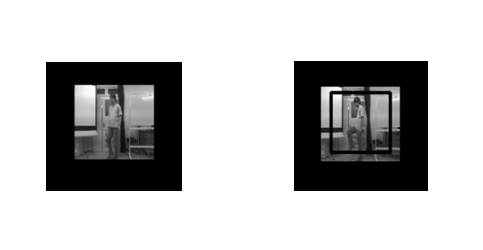
\includegraphics[width=9cm]{image/ninshiki.png}
  \caption[カスケード分類器を用いたサッカーモードのユーザ認識]{カスケード分類器を用いたサッカーモードのユーザ認識.}
\label{lbpfig}
\end{figure}
\vspace{1cm}
ユーザAとユーザBのサッカーモードにおける動作をフレームで抜き出して,
作成したカスケード分類器の認識率?を評価する.
\begin{table}[htb]
  \centering
   \begin{tabular}{ccccc}	\hline
     分類器 & ポジティブ画像 & ネガティブ画像 & ステージ数 & maxFalseAlarmRate\\	\hline \hline
     A & 1200 & 345 & 7 & 0.7\\
     B & 1200 & 345 & 8 & 0.65\\
     C & 1200 & 345 & 9 & 0.6\\
     D & 1200 & 345 & 13 & 0.5\\
     E & 1200 & 345 & 14 & 0.35\\\hline
   \end{tabular}
  \caption[評価実験に用いたカスケード分類器]{評価実験に用いたカスケード分類器.}
\end{table}
\clearpage
\section{評価結果}
\begin{table}[htb]
  \centering
   \begin{tabular}{cccc}	\hline
     分類器 & 認識? & 誤認識? \\	\hline \hline
     A & & \\
     B & & \\
     C & & \\
     D & & \\
     E & & \\\hline
   \end{tabular}
  \caption[評価結果]{評価結果.}
\end{table}
\end{comment}